\chapter{Definitions and datasets\label{chap::def}}

Trees are partitioned into hierarchical elements with definitions that may vary between Forest Inventories and datasets (\eg Fig. \ref{fig::partition}).

\begin{figure*}[h]
	\centering
	\begin{tikzpicture}
	%% Level 0
	\node (orig) at (0, 0) {Whole tree};
	
	%% Level 1
	\node[below right = of orig] (belowground) {Below-ground};
	\node[above right = of orig] (aboveground) {Above-ground};
	
	%% Level 2
	\node[above right = of aboveground] (stem) {Main stem};
	\node[right = of aboveground] (lat) {Lateral};
	\node[below right = of aboveground] (fol) {Foliage};
	
	\node[right = of belowground] (root) {Root};

	%% Level 3
	\node[above right = of stem] (stemtop) {Stem top};
	\node[right = of stem] (bole) {Bole};
	\node[below right = of stem] (stump) {Stump};

	\node[below right = of lat] (lbranch) {Large branches};
	\node[above right = of lat] (sbranch) {Small branches};

	\begin{scope}[on background layer] % From background library
		% \fill[lightGrey] (2.735294,0) rectangle (6,6);
		\node[fit=(belowground)(aboveground), fill = lightGrey, inner sep=5mm] {};
	\end{scope}

\end{tikzpicture}
	\caption{Hierarchical elements of trees, figure inspired by \cite{Gschwantner2009} \label{fig::partition}}
\end{figure*}

In our case, the tree data come from different institutes, different periods of time, and do not all have the same tree components recorded:

\begin{marginfigure}%
	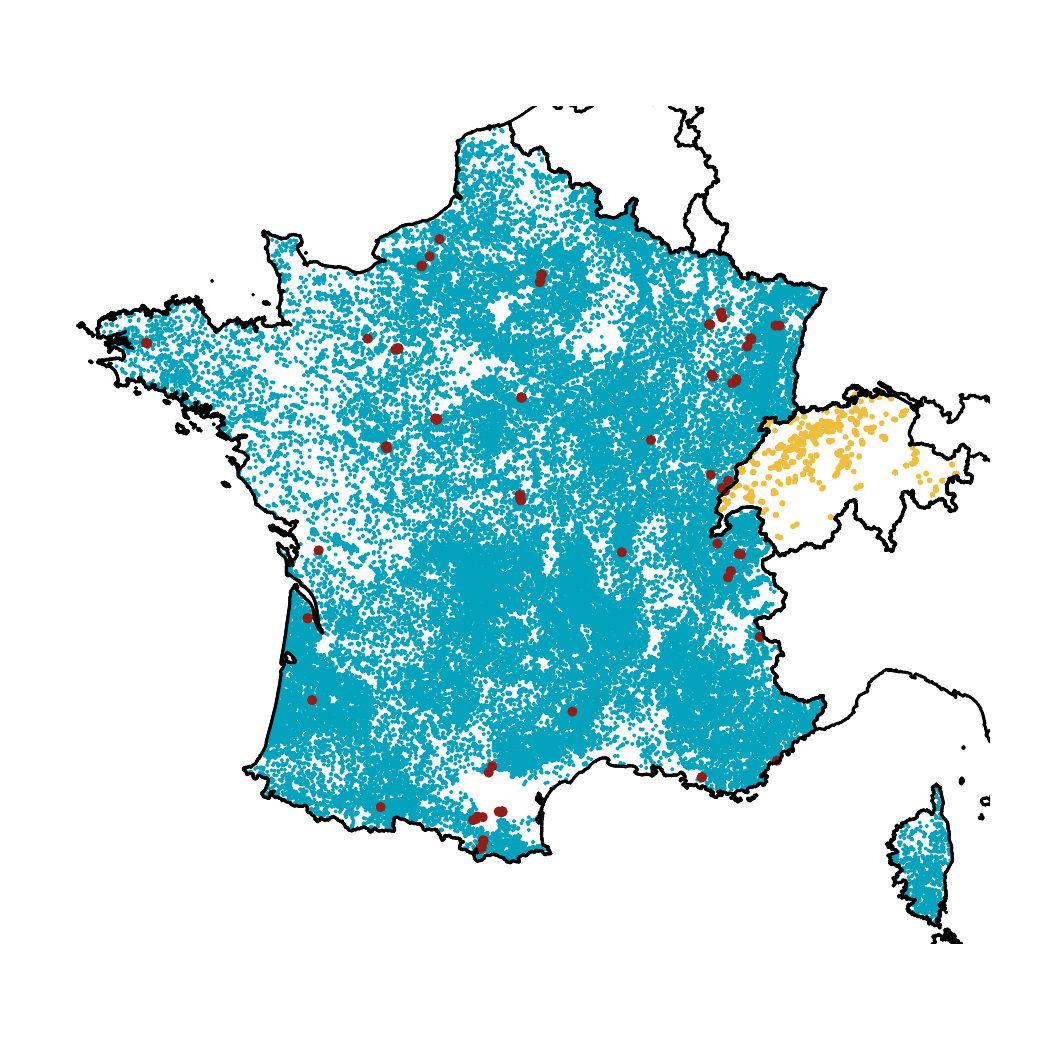
\includegraphics[width=\marginparwidth]{./Figures/map.png}
	\caption{Plot location for French \NFI, Emerge, and Swiss dataset.\label{fig::map}}
\end{marginfigure}

\begin{enumerate}
	\item `Protocole Oudin', dataset preserved by INRAE, ranging from 1930 to 1980 (in red on Fig. \ref{fig::map}). Recorded, the bole volume, and the large and small branches.
	\item The French \NFI (in blue on the Fig. \ref{fig::map}). Data range from 1988 to 2007 (data before 1988 record diameter rather than circumference). Recorded the bole volume.
	\item The `Office National des Forêts (ONF)', with protocols from 1972 and from 1983 (not used as there is no coordinates)
	\item Institut Technologique Forêt, Cellulose, Bois-construction, Ameublement (FCBA), not used so far for the aerial volume
	\item L'Institut pour le développement forestier (IDF) which is the R\&D of the Centre National de la Propriété Forestière and the Institut national de recherche en sciences et technologies pour l'environnement et l'agriculture (IRSTEA, currently INRAE)
\end{enumerate}

We decided to use the definitions from \cite{Gschwantner2009} (see Figs. \ref{fig::partition} and \ref{fig::ign_tree}):

\begin{marginfigure}%
	\begin{tikzpicture}
	\node (tree) at (0, 0) {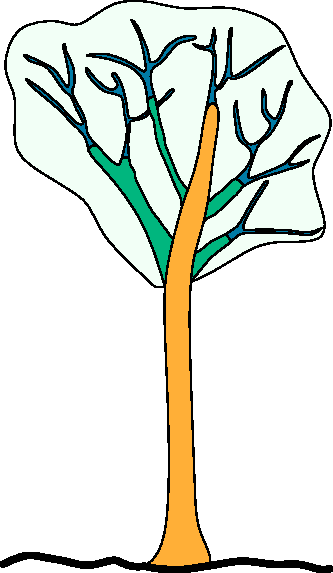
\includegraphics[width=\marginparwidth]{./Figures/ign_tree.pdf}};
	\matrix[below = -0.2cm of tree] {
		\node [draw, shape = rectangle, fill = egyptYellow, label = right:Bole] {}; \\
		\node [draw, shape = rectangle, fill = egyptGreen, label = right:Large branches] {}; \\
		\node [draw, shape = rectangle, fill = egyptBlue, label = right:Small branches] {}; \\
	};
\end{tikzpicture}
	\caption{Scheme of tree components.\label{fig::ign_tree}}
\end{marginfigure}

\begin{itemize}
	\item Main stem: The stem of a tree is the above-ground part of the main (off) shoot with apical dominance
	\begin{itemize}
		\item Stem top: topmost part of the stem from an over-bark base-diameter of \qty{7}{\centi\metre} (French \NFI) to the stem tip
		\item Bole: above-ground part of the stem between stump and the stem top
		\item Stump: above-ground base part of the stem which would remain after a tree was cut under normal felling practices
	\end{itemize}
	\item Lateral parts:
	\begin{itemize}
		\item Large branches: portion of the above-ground lateral parts with a diameter of more than or equal to \qty{7}{\centi\metre} (French \NFI)
		\item Large branches: portion of the above-ground lateral parts with a diameter of less than \qty{7}{\centi\metre} (French \NFI)
	\end{itemize}
\end{itemize}
